\documentclass[brazil]{beamer}
\usepackage[utf8]{inputenc}
\usepackage[T1]{fontenc}
\usepackage[brazil]{babel}  % idioma
\usepackage{lmodern}
\usepackage{graphicx}			%para imagens
\usepackage{epstopdf} 			%resolve problemas eps-pdf
\usepackage{fancyhdr}			% para o cabeçalho bonito
\usepackage{caption}				%para legendas
\usepackage{placeins} 			%controlar o lugar dos floats
\usepackage{color}
\usepackage{url}
\usepackage{bm}
\renewcommand{\UrlFont}{\tiny}
\usepackage{relsize}
\usepackage{hyperref}

\usetheme{Dresden}
\usecolortheme{orchid}
\setbeamertemplate{navigation symbols}{}

\newcommand{\HRule}{\rule{\linewidth}{0.5mm}}

\title{EZ3D: Rastreamento Visual de Movimentos Faciais sem Marcadores para Modelos de Animação Tridimensionais}
\author{Juarez Aires Sampaio Filho \\ Rodrigo de Assis Ramos Lima}
\titlegraphic{\leavevmode\smash{\raisebox{6.5cm}{
\includegraphics[width=0.7\textwidth]{./img/logo.jpg}}}}
\institute{Universidade de Brasília}
\date{8 de Dezembro de 2016}


\begin{document}
\begin{frame}
        \titlepage
\end{frame}

\begin{frame}[fragile]
  \frametitle{Conteúdo}
  \begin{itemize}
     \item Introdução
     \begin{itemize}
     	\item O Mercado de Animação
     	\item Técnicas para Transferência de Movimentos
    	 	\item Motivação
   	 \end{itemize}
     \item Metodologia Utilizada
     \begin{itemize}
    	 	\item Rastreamento de Pontos do Rosto
    	 	\item Estimação de Tridimensionalidade e Filtros Digitais
    	 	\item Mistura de Poses
   	 \end{itemize}
     \item Resultados
     \begin{itemize}
    	 	\item Rastreamento de Pontos do Rosto
    	 	\item Estimação de Tridimensionalidade e Filtros Digitais
    	 	\item Resultado Final
   	 \end{itemize}
     \item Conclusões
  \end{itemize}
\end{frame}

\section{Introdução}
\begin{frame}[fragile]
  \frametitle{Introdução}

  \begin{definition}
  Animação Computacional é a arte de criar imagens em movimento pelo uso de
computadores.
%%https://www.sciencedaily.com/terms/computer_animation.htm
  \end{definition}
      \begin{figure}
        \centering
        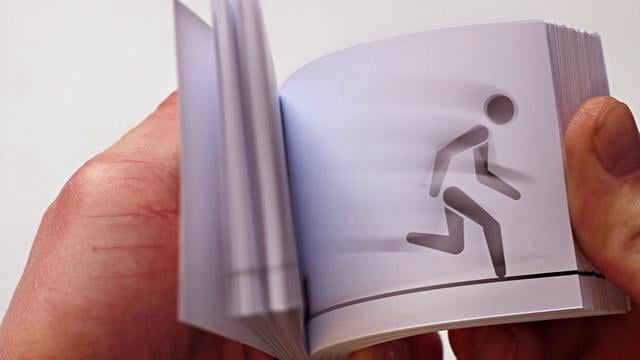
\includegraphics[width = 0.6\textwidth, keepaspectratio]{./img/flipBook.jpg}
        \caption{A técnica de animação dá vida aos modelos ao posicioná-los em
          poses ligeiramente diferentes, criando a ilusão do movimento }
      \end{figure}


\end{frame}


\begin{frame}
  Animações computacionais são utilizadas em filmes completamente digitalmente
  animados.
      \begin{figure}
        \centering
        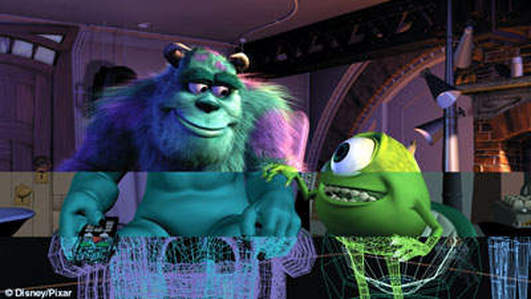
\includegraphics[width = 0.8\textwidth, keepaspectratio]{./img/sully.jpg}
        \caption{Um único quadro com o personagem Sully custou em média de 11 a 12 horas de trabalho criativo.}
      \end{figure}
\end{frame}

\begin{frame}
  Ou também para compor filmes onde atores interagem com modelos computacionais.
      \begin{figure}
        \centering
        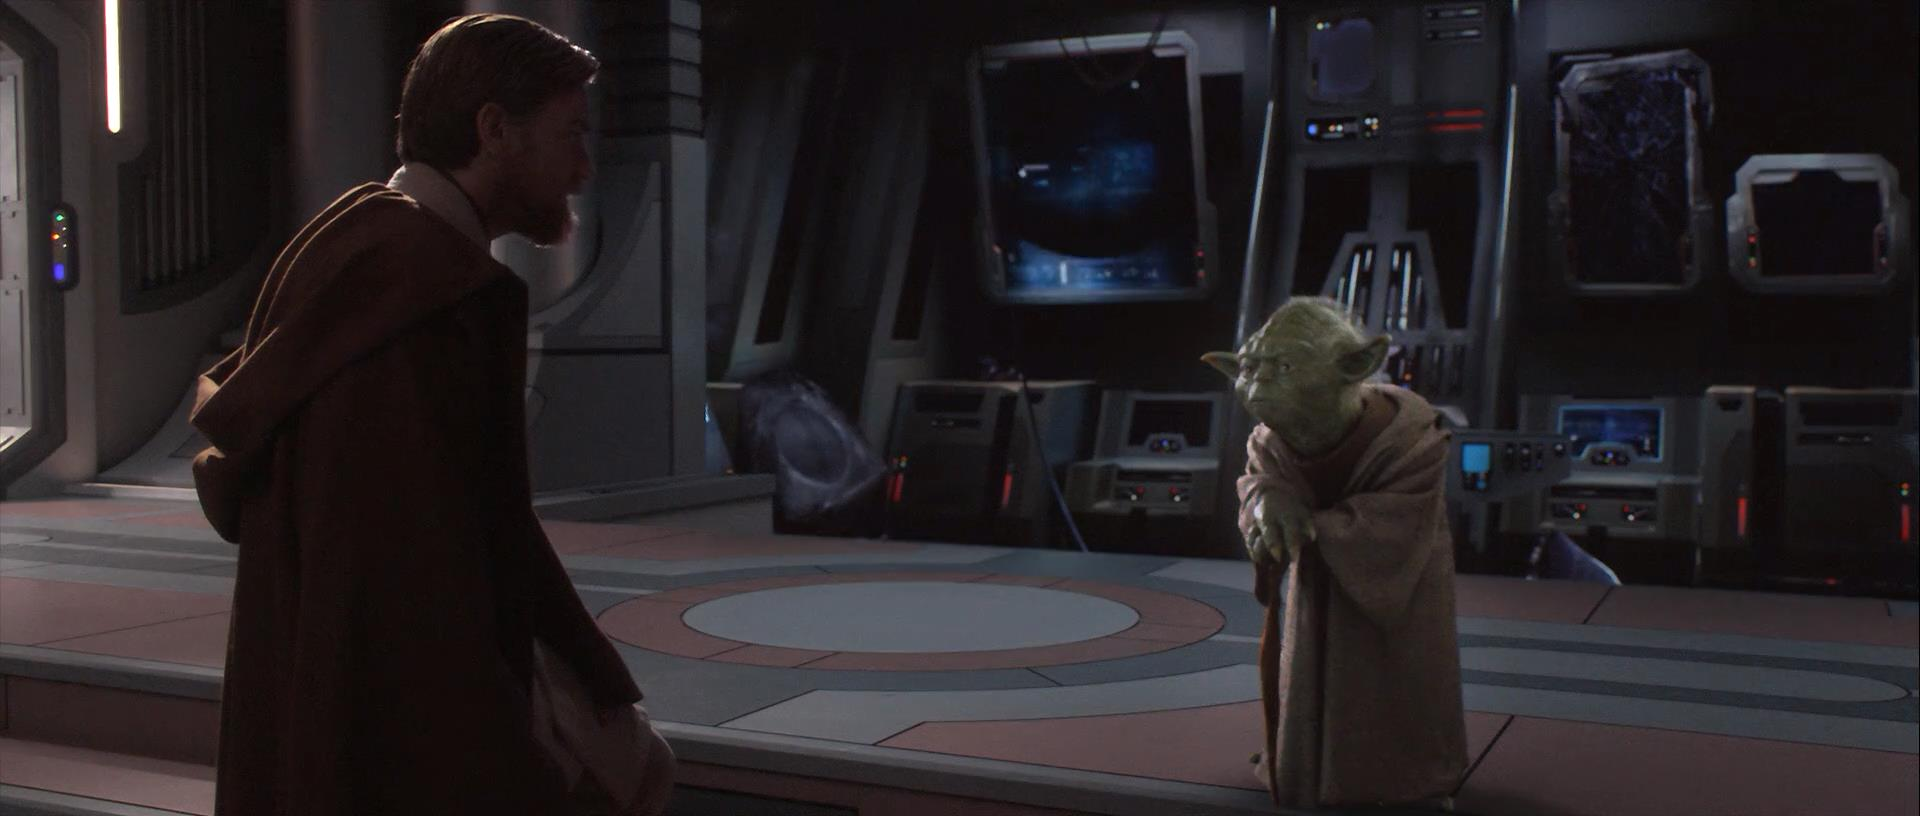
\includegraphics[width = 0.8\textwidth, keepaspectratio]{./img/actorAndAnimation.jpg}
        \caption{O ator interage com personagem completamente digital.}
      \end{figure}
\end{frame}

\begin{frame}
  É possível também transferir movimentos de atores para modelos
  \begin{figure}[ht]
        \begin{minipage}[b]{0.45\linewidth}
            \centering
            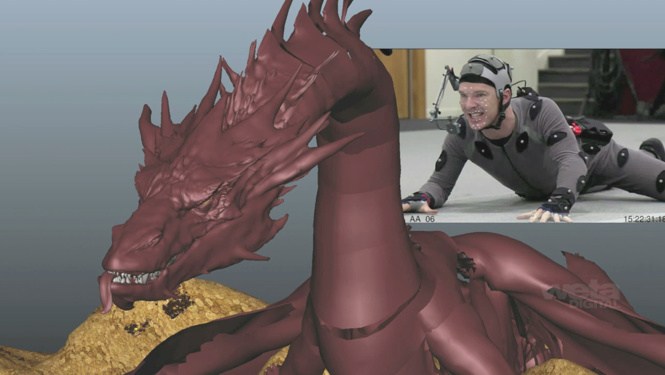
\includegraphics[width = 1.0\textwidth, keepaspectratio]{./img/smaug_left.jpg}
        \end{minipage}
        \begin{minipage}[b]{0.45\linewidth}
          \centering
              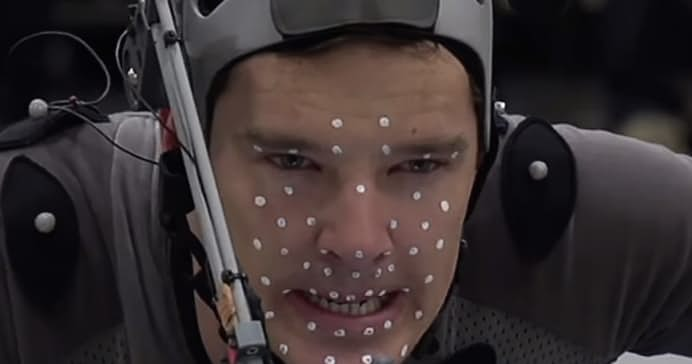
\includegraphics[width = 1.0\textwidth, keepaspectratio]{./img/smaug_right.jpg}
        \end{minipage}

        \caption{Movimentos e expressões são transferidos do ator para o modelo.
       Artistas gráficos dão o retoque final na animação para garantir que o
     resultado seja o mais convincente possível. }
      \end{figure}
\end{frame}


\begin{frame}
  \begin{itemize}
      \item Motivação:
      \begin{itemize}
        \item os produtos existente apresentam \textbf{alto custo}: 
          \begin{itemize}
            \item inúmeras horas de trabalho artístico
            \item equipamentos especias de captura
            \item ambientes controlados
          \end{itemize}
        \item Esse custo pode se tornar proibitivo para aplicações
          independentes que não dispõe do mesmo orçamento que blockbusters.
      \end{itemize}   
      \item Será que é possível desenvolver um sistema de baixo custo que
        realize transferência de movimento para um avatar computacional?
  \end{itemize} 

\end{frame}


\section{Metodologia}

\subsection{Inspiração}
\begin{frame}
	\frametitle{Vídeo sobre Blend Shapes no Maia}
      \begin{figure}
        \centering
        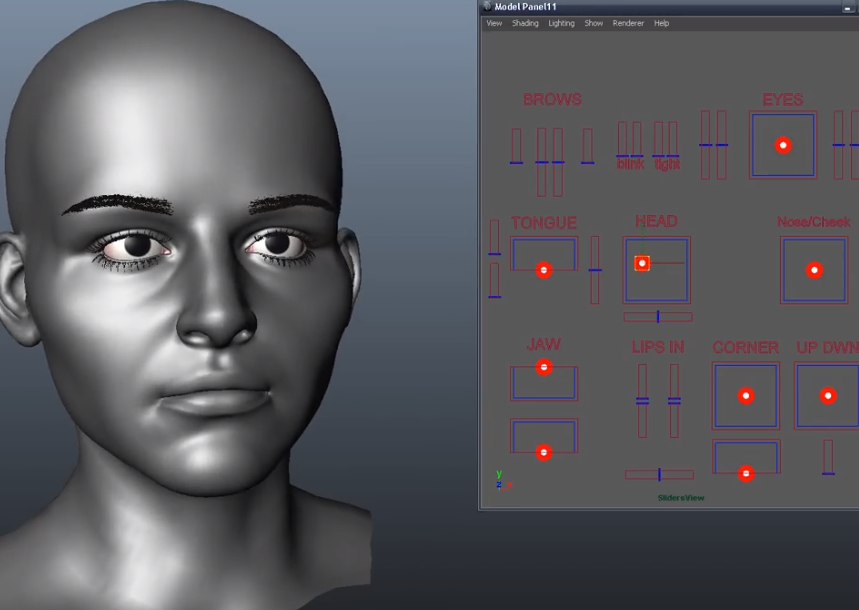
\includegraphics[width = 0.8\textwidth, keepaspectratio]{./img/maiaDemo.png}
      \end{figure}   
\end{frame}


\begin{frame}
	\frametitle{Metodologia}
      \begin{figure}
        \centering
        \includegraphics[width = 0.445\textwidth, keepaspectratio]{./img/TG-metodologia-correta-2.png}
      \end{figure}   
\end{frame}

\begin{frame}
\frametitle{Rastreamento de Pontos do Rosto}
  \begin{itemize}
      \item Algoritmo Simplificado:   
          \begin{figure}
        \centering
        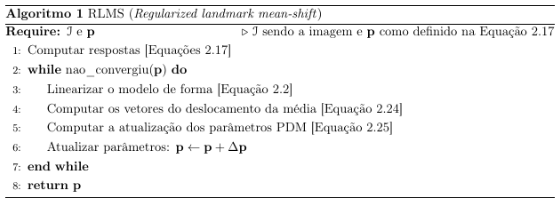
\includegraphics[width = 0.8\textwidth, keepaspectratio]{./img/algorithm.png}
      \end{figure}
  \end{itemize} 
\end{frame}

\begin{frame}
\frametitle{Estimação de Tridimensionalidade}
  \begin{itemize}
      \item Triangulação:
      
      \begin{figure}
        \centering
        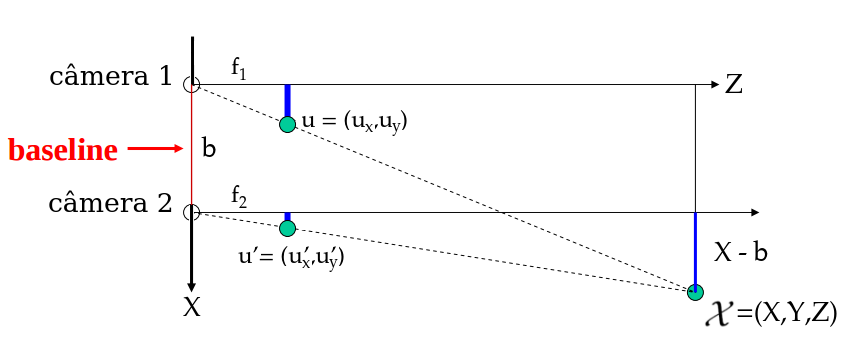
\includegraphics[width = 0.8\textwidth, keepaspectratio]{./img/TG_triangulation_pdf_washington_pt2.png}
      \end{figure}
      
      $X = (u_x/f_1)  Z$ ou $ X = (u'_x/f_2)  Z + b $
      
      $Y = (u_y/f_1) Z$ ou $ Y = (u'_y/f_2) Z$
      
      $Z = f_1  f_2  b / (u_x  f_2 - u'_x  f_1)$
      
      \item Calibração dos Parâmetros Intrínsecos:
  \end{itemize} 
\end{frame}

\begin{frame}
\frametitle{Filtros}
  \begin{itemize}
      \item Resposta finita ao Impulso: 
      
      $\gamma(n) = 	\sum_{i=0}^{\mathcal{M}} b_i \chi(n-i)$
      
      \item Pela técnica da Janela: 
      

  \end{itemize} 
\end{frame}

\begin{frame}
\frametitle{Mistura de Poses}
  \begin{itemize}
  	
  	\item Blend Shapes:
  	
  	A técnica de Mistura de Poses - MP, do inglês \textit{Blend Shapes} ou \textit{Morph Target}, é uma das opções comumente empregadas para animar objetos deformáveis como a \textbf{face humana}.
  	
 	 	\begin{itemize}
  	
 	 	\item Definição:
  	
 	 	A técnica consiste em gerar poses intermediárias como uma \textbf{combinação linear} de poses pré-definidas. Os modelos que representam as poses chaves devem ter a \textbf{mesma quantidade de vértices}.
  	
  	
  	    \item Equação para a Renderização de uma pose $J$:
      
   		   $J = \sum_{i=1}^L  w_i M_i$
      
   		   $J = M_1 + \sum_{i = 2}^L w_i \Delta M_i $

  \end{itemize} 

  \end{itemize} 
\end{frame}

\begin{frame}
\frametitle{Resultados}
  \begin{itemize}
      \item Rastreamento de Pontos do Rosto:
      
       \begin{figure}
        \centering
        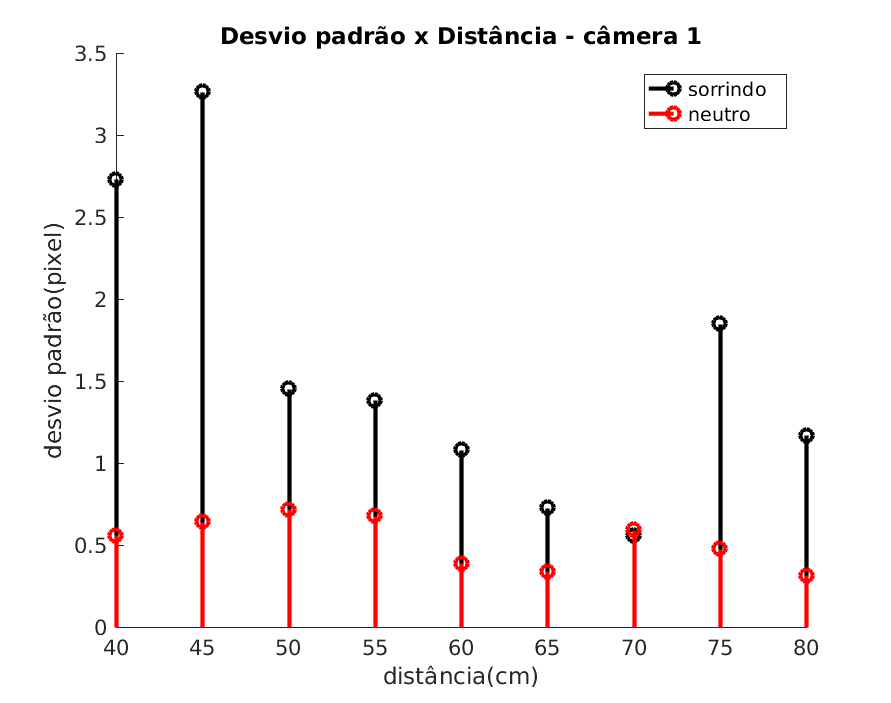
\includegraphics[width = 0.6\textwidth, keepaspectratio]{./img/desvio_cameraEsquerda.jpg}
      \end{figure}
          
  \end{itemize} 
\end{frame}

\begin{frame}
\frametitle{Resultados}
  \begin{itemize}
      \item Rastreamento de Pontos do Rosto:
      
       \begin{figure}
        \centering
        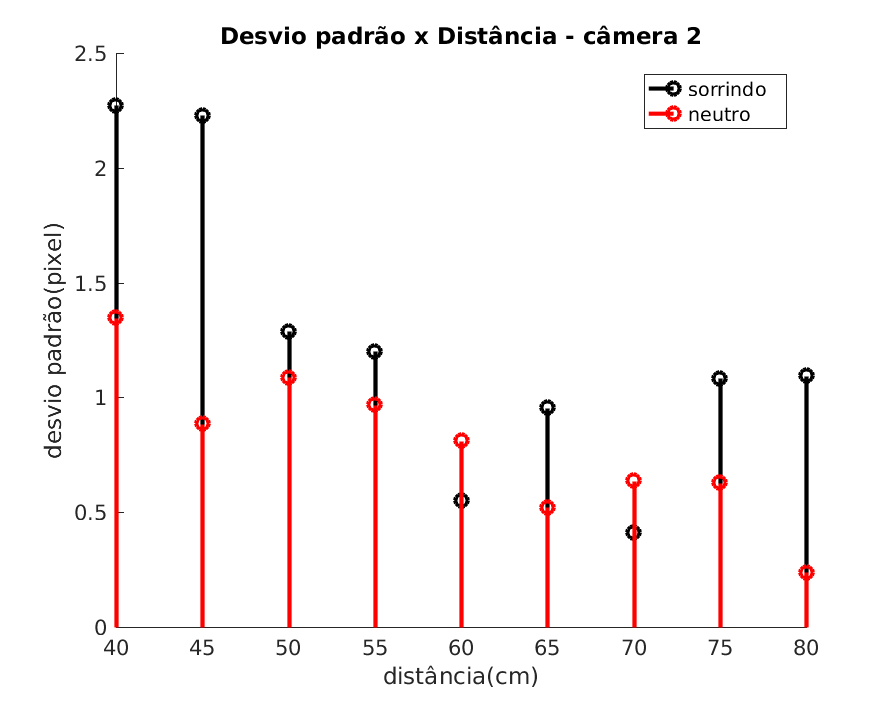
\includegraphics[width = 0.6\textwidth, keepaspectratio]{./img/desvio_cameraDireita.jpg}
      \end{figure}
          
  \end{itemize} 
\end{frame}

\begin{frame}
\frametitle{Estabilização do Rastreamento}
  \begin{itemize}
      \item Estimação da Tridimencionalidade:
      \begin{figure}
        \centering
        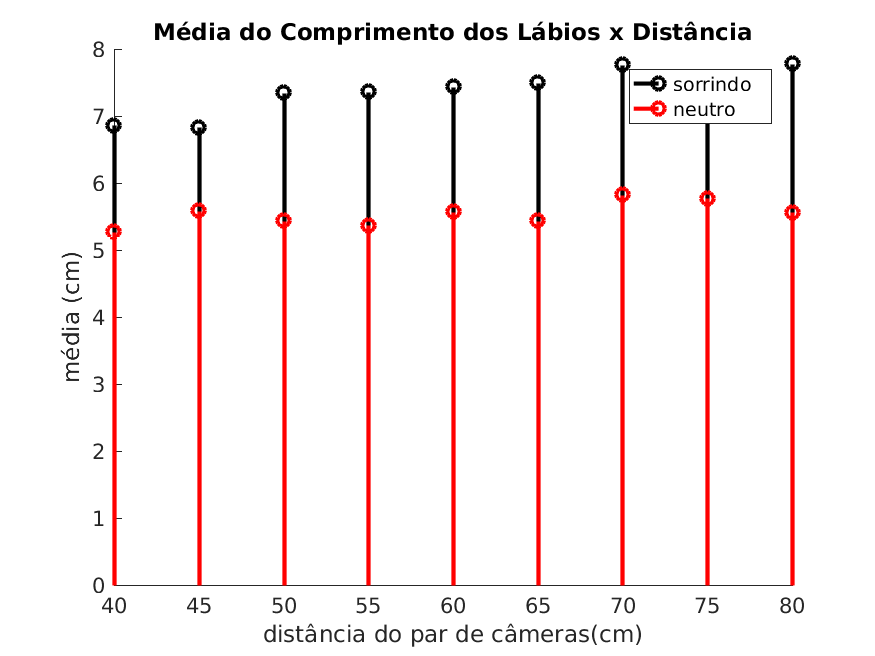
\includegraphics[width = 0.6\textwidth, keepaspectratio]{./img/media_3d.png}
      \end{figure}
               
  \end{itemize} 
\end{frame}

\begin{frame}
  \begin{itemize}
      \item Filtros:
      \begin{figure}
\centering
\begin{tabular}{c}
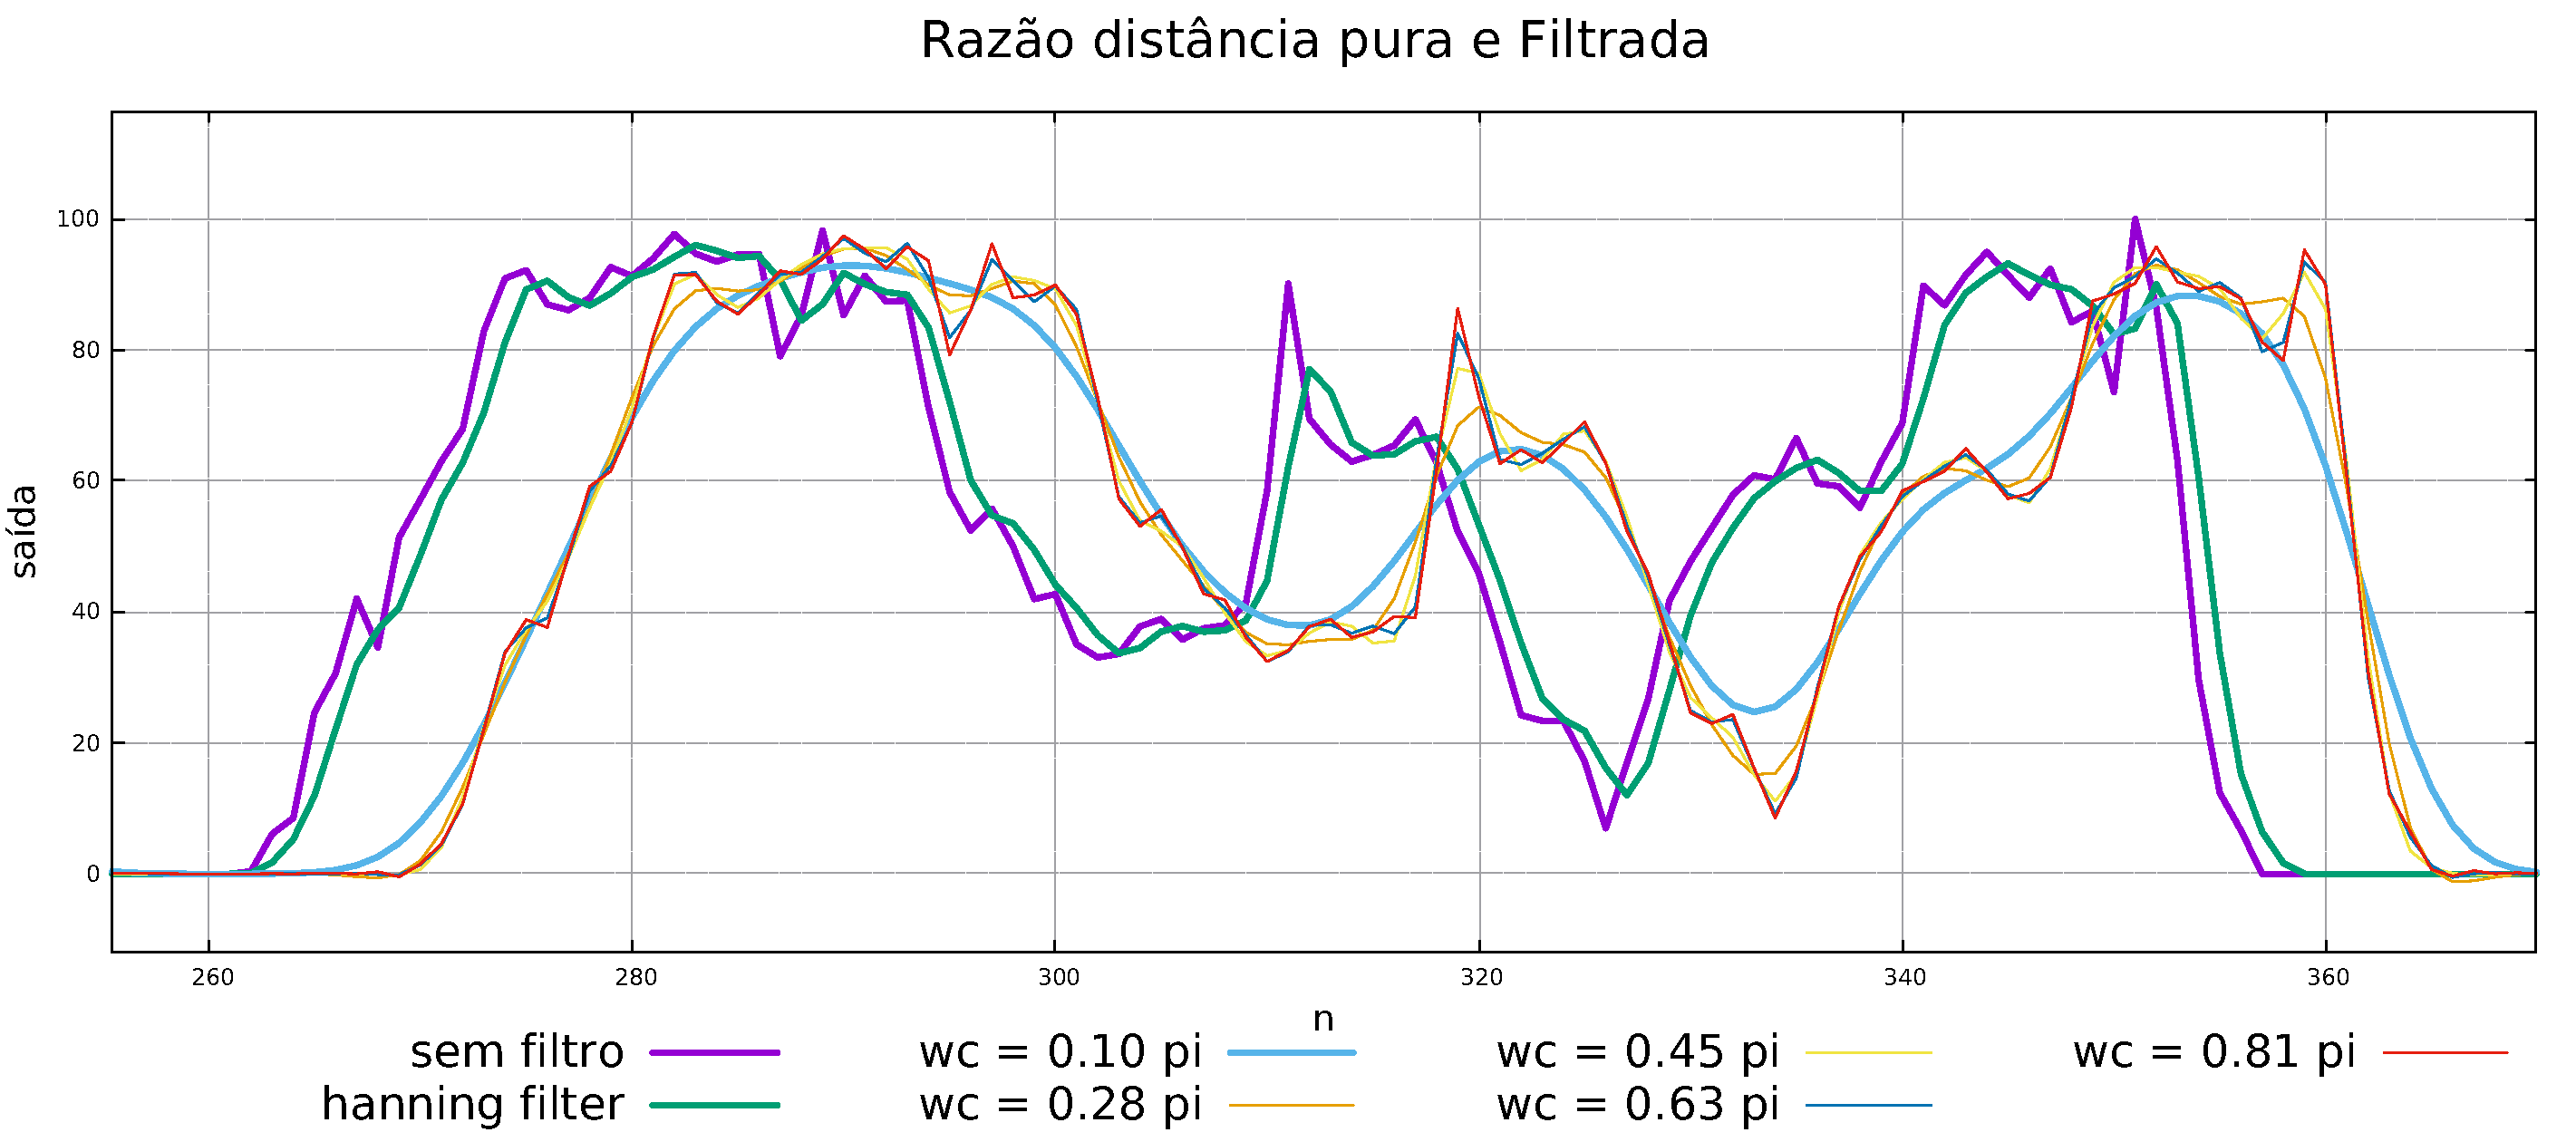
\includegraphics[width=0.6\linewidth]{./img/filter-result-left-eye.pdf} \\
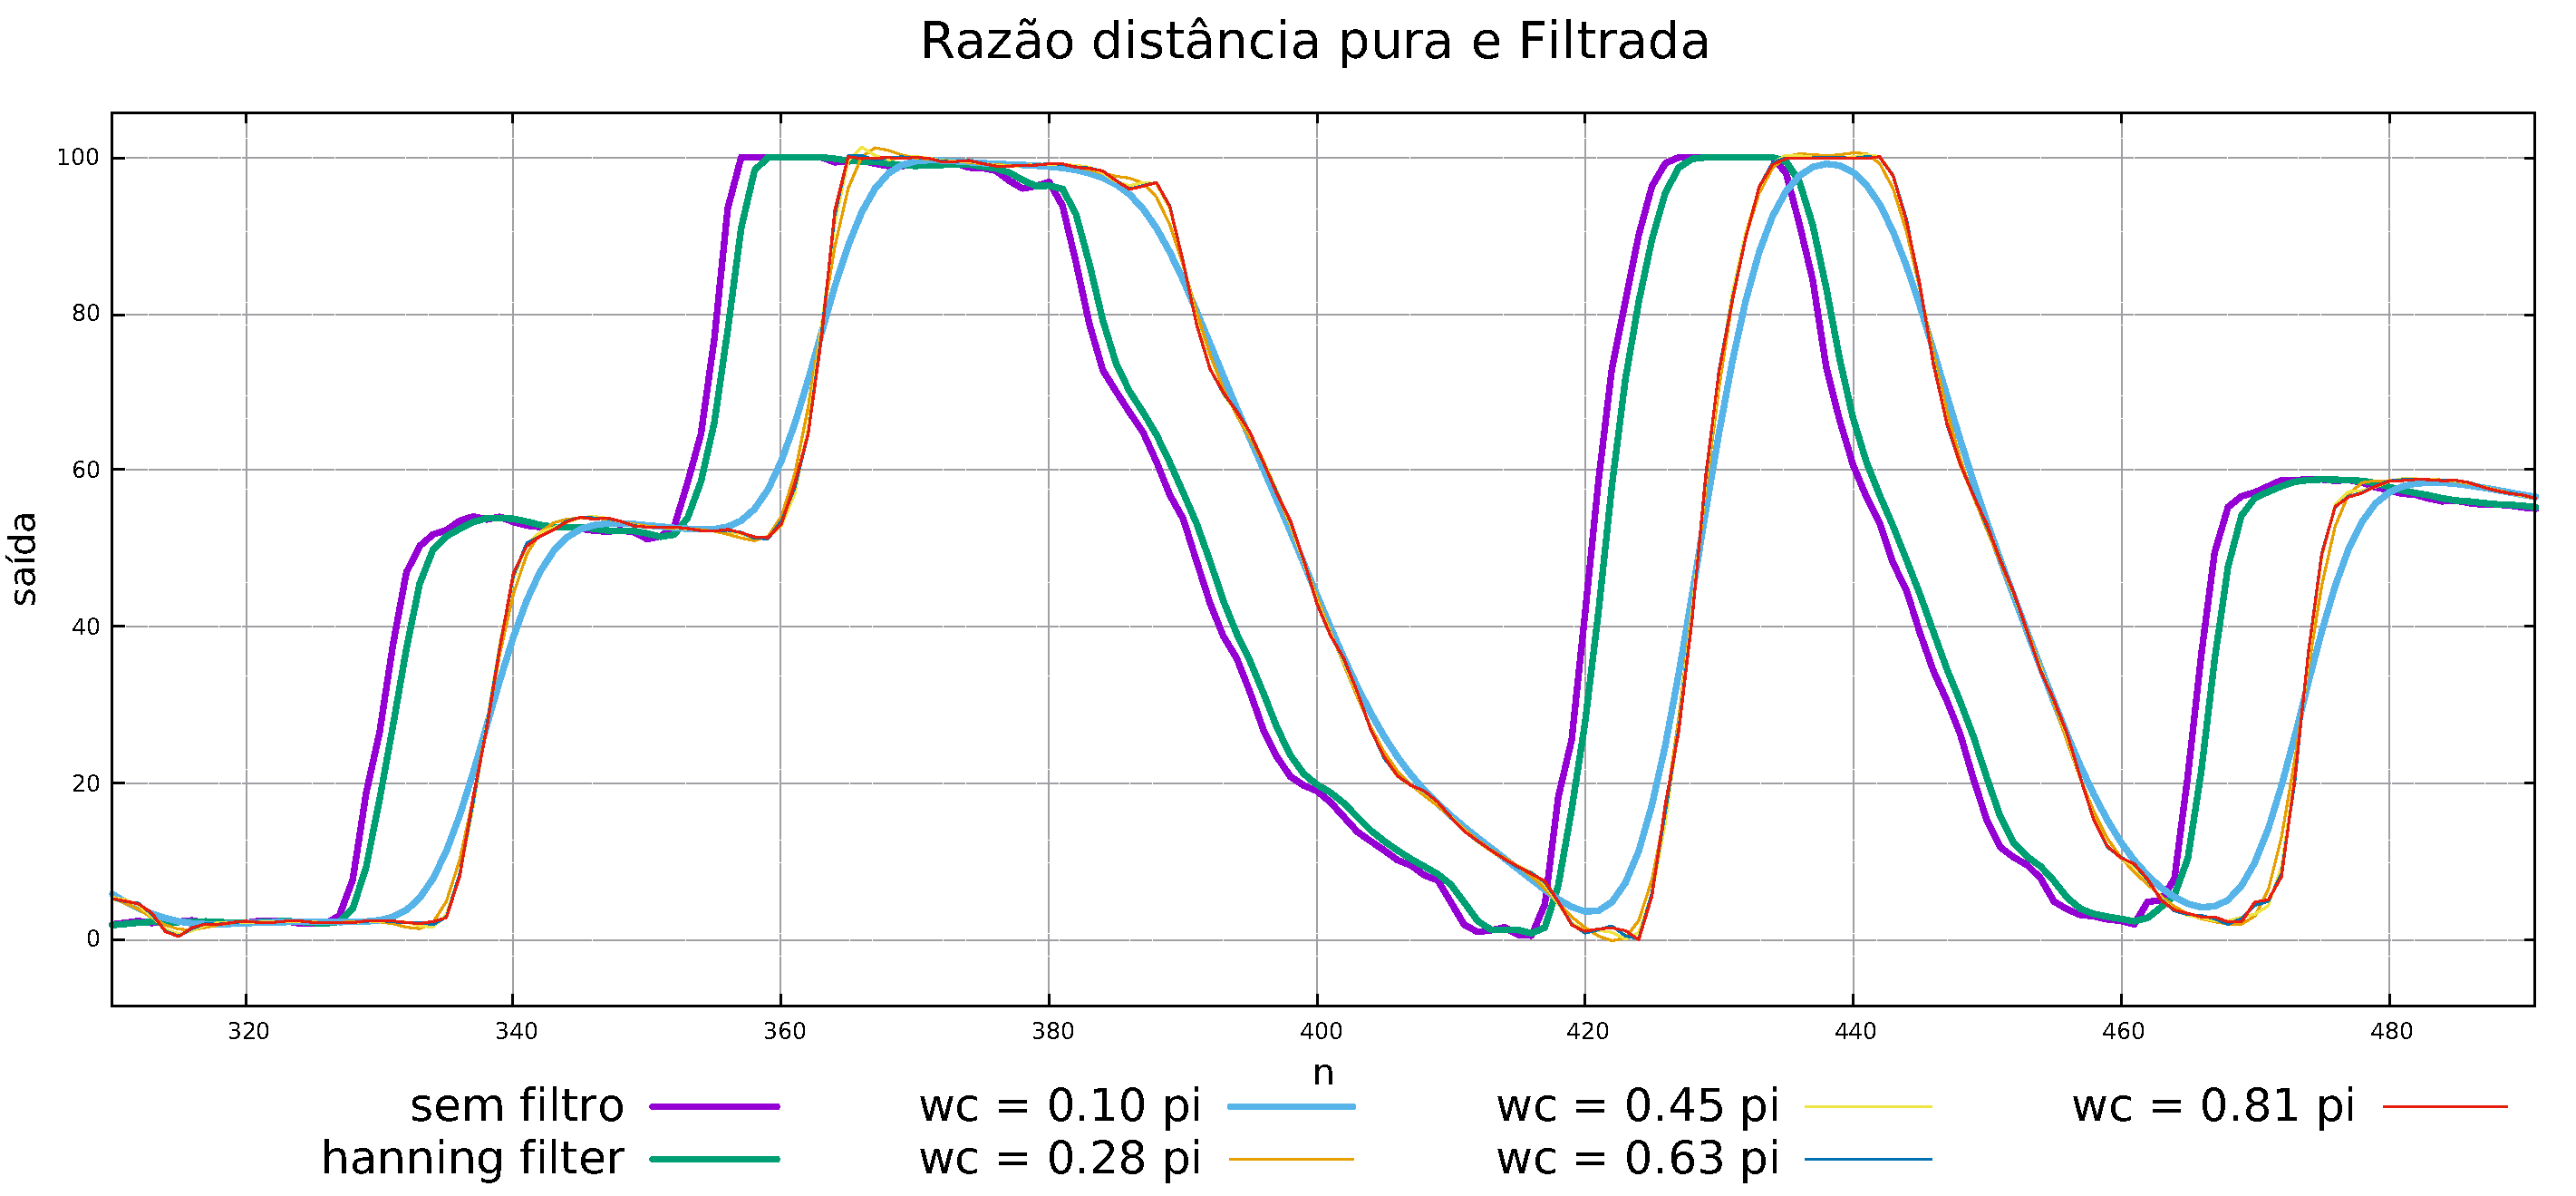
\includegraphics[width=0.6\linewidth]{./img/filter-result-open-mouth.pdf} \\
\end{tabular}
\caption{Resultado da resposta ao sinal dos filtros projetados para o movimento do olho esquerdo e da boca}
\end{figure}
              
  \end{itemize} 
\end{frame}

\begin{frame}
  \begin{itemize}
      \item Filtros:
	\begin{figure}
        \centering
        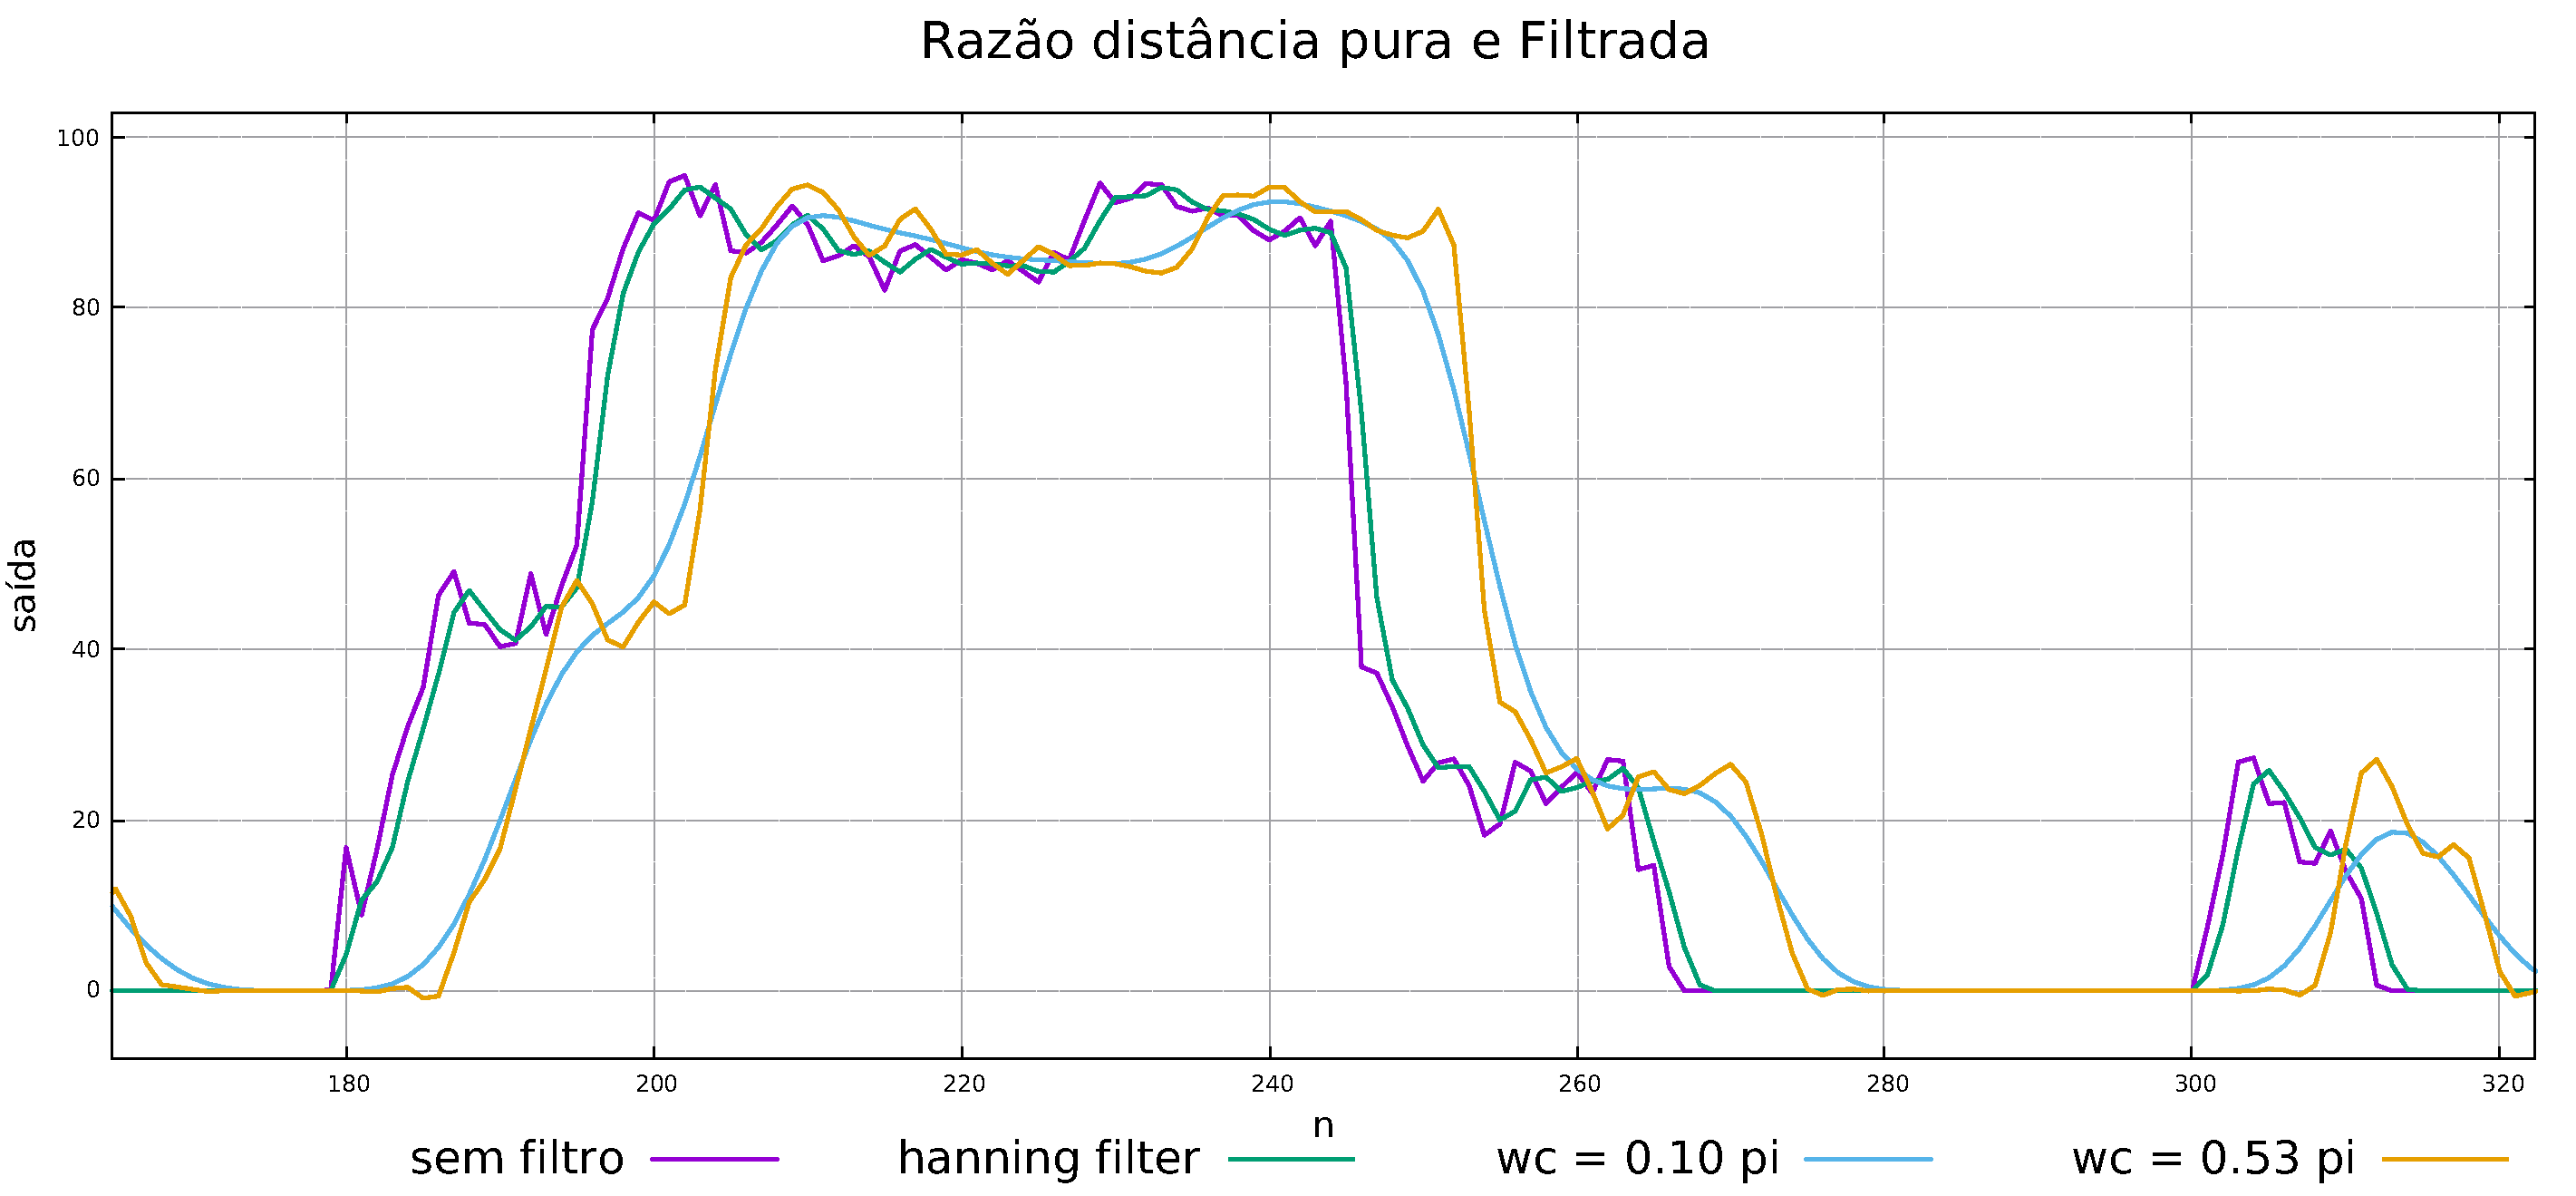
\includegraphics[width = 0.8\textwidth, keepaspectratio]{./img/filter-result-smile.pdf}
      \end{figure}
              
  \end{itemize} 
\end{frame}

\begin{frame}
  \begin{itemize}
      \item Resultado Final:
              
  \end{itemize} 
\end{frame}


\begin{frame}
\frametitle{Conclusões}
  \begin{itemize}
      \item Análise:
      
      \item Trabalhos Futuros:
              
  \end{itemize} 
\end{frame}


\end{document}
